% interactnlmsample.tex
% v1.05 - August 2017

\documentclass[]{interact}

\usepackage{epstopdf}% To incorporate .eps illustrations using PDFLaTeX, etc.
\usepackage[caption=false]{subfig}% Support for small, `sub' figures and tables
%\usepackage[nolists,tablesfirst]{endfloat}% To `separate' figures and tables from text if required
%\usepackage[doublespacing]{setspace}% To produce a `double spaced' document if required
%\setlength\parindent{24pt}% To increase paragraph indentation when line spacing is doubled

\usepackage{tikz}
\usepackage{pdfpages}
\usepackage{pgfplots}
\usepackage{verbatim}
\usepackage{dirtytalk}

\usepackage[numbers,sort&compress]{natbib}% Citation support using natbib.sty
\bibpunct[, ]{[}{]}{,}{n}{,}{,}% Citation support using natbib.sty
\renewcommand\bibfont{\fontsize{10}{12}\selectfont}% Bibliography support using natbib.sty
\makeatletter% @ becomes a letter
\def\NAT@def@citea{\def\@citea{\NAT@separator}}% Suppress spaces between citations using natbib.sty
\makeatother% @ becomes a symbol again

\theoremstyle{plain}% Theorem-like structures provided by amsthm.sty
\newtheorem{theorem}{Theorem}[section]
\newtheorem{lemma}[theorem]{Lemma}
\newtheorem{corollary}[theorem]{Corollary}
\newtheorem{proposition}[theorem]{Proposition}

\theoremstyle{definition}
\newtheorem{definition}[theorem]{Definition}
\newtheorem{example}[theorem]{Example}

\theoremstyle{remark}
\newtheorem{remark}{Remark}
\newtheorem{notation}{Notation}

\begin{document}

\articletype{ARTICLE TEMPLATE}% Specify the article type or omit as appropriate

\title{Article Title}

\author{
\name{A.~N. Author\textsuperscript{a}\thanks{CONTACT A.~N. Author. Email: latex.helpdesk@tandf.co.uk} and John Smith\textsuperscript{b}}
\affil{\textsuperscript{a}Taylor \& Francis, 4 Park Square, Milton Park, Abingdon, UK; \textsuperscript{b}Institut f\"{u}r Informatik, Albert-Ludwigs-Universit\"{a}t, Freiburg, Germany}
}

\maketitle

\begin{abstract}
Abstract
\end{abstract}

\begin{keywords}
Computational intelligence, real-time strategy
games, planet wars, artificial immune system, particle swarm optimization.
\end{keywords}


\section{Introduction}
% no \IEEEPARstart
Strategy video game is to make a decision under a set of units during the game. A real-time Strategy game is a sub-genre of strategy game, where players move (control multiple structures) in real time. Moreover, RTS game is a complex competitive domain where allowed to virtualize battles against players with a purpose of destroying other enemies units or to generate more self-units to secure an area.\cite{doc5}

The complex nature of these games makes their conception more challenging because : 
\begin{itemize}
  \item Their real-time nature: the player has to move without waiting for other players to act.
  \item The player has to control a large number of units simultaneously.
  \item Make a decision under uncertainty: partial observability, time need to move, units need to react, ...etc.
\end{itemize}


Recent development in the field of RTS video games led to making the paradigm of Artificial Intelligence as a key instrument in the designing of the agents(bots), that will react in a real scenario against other players during the game. In addition, the RTS games posing new challenges to AI and it is a wide area to test AI concepts and methodologies.\cite{doc5,doc1,doc2,doc3,doc4}

The bot's design makes a significant challenge to RTS games conception process. A bot is an autonomous agent act with human player in a real scenario under any computer-based framework. \cite{doc4}In the other hand, the huge progress of video games and their international competitions, it's becoming extremely difficult to ignore the existence of human expert players and their experience within the conception of bot's behavior. While, including expert experimentation under conception process will make the bot more challenging and hard to beat that implies more challenging game and more interesting.\cite{doc3}

Google Artificial Intelligence (GAIC) Challenge is one of the international RTS game competition that was sponsored by Google Community in 2010. In this competition, Google chooses planet war as a competitive RTS game. While this paper will study planet war game as a subject. Planet war is an RTS game which simulates battles against autonomous agents under several situations (maps) with the aim of winning the game by owning the maximum number of planets.


The bot concept plays a critical role in RTS game progression, designing a challenging bot mean designing a challenging game. In case of planet war, a set of pre-determined parameters need to make the bot under real game. Moreover, the parameters selection will affect the behavior of the bot later, so, good selection process led to the better reaction during the game. In the other hand, the previous parameters it's a large research area that treated as an optimization itself.\cite{doc1}. However, the selection process is trying to find the most important parameters for best bot performance\cite{doc1}.

The specific objective of this study was to design a planet war bot using an Evolutionary Algorithm named Artificial Immune System (AIS) to determine parameters weights (values) by maximizing an objective function based on turns number played by the bot and the number of wins.

The paper has been organized in the following way: First of all, this paper gives a brief description of planet war and all rules applied during the game. In the second section, AIS algorithm was defined. The third chapter concerned with the approach used for this study by defining the global architecture of the bot. In the remaining part, all experimental results are presented.\\

\section{Planet War}

As we mentioned previously one of the international competition was organized by google community. In this pager, we worked with planet war game chosen as RTS game in this competition with the aim of designing a fighter bot. During a planet war\cite{doc1}, firstly you have to choose a map to run a match, each map has a number of distributed planets in different positions with a specific number emerged the starships amount situated in the planet. Each planet in the map owned by player, opponent or neutral (owned by no one), moreover, each planet owner by players will increase the number starship per turn based on their growth rate except the neutral planets that will not be able to generate new additional starships. The main purpose of planet war\cite{doc1} is to compete with other players and try to beat all of them during the game by limited turns number.  \\

Moreover, the planet war fighter bot face two important problems that make the agent's conception more challenging:
The first problem \cite{doc1} that the bot can bot save any previous stats from previous turns as actions it made, map state...etc. Since in each turn, bot finds under an unknown map the same thing when it begins the game in the first time. The second problem\cite{doc3} in inherited by the RTS game nature that is shown as the time required to act (make an action) is defined by 1 second.

\begin{figure}
\centering
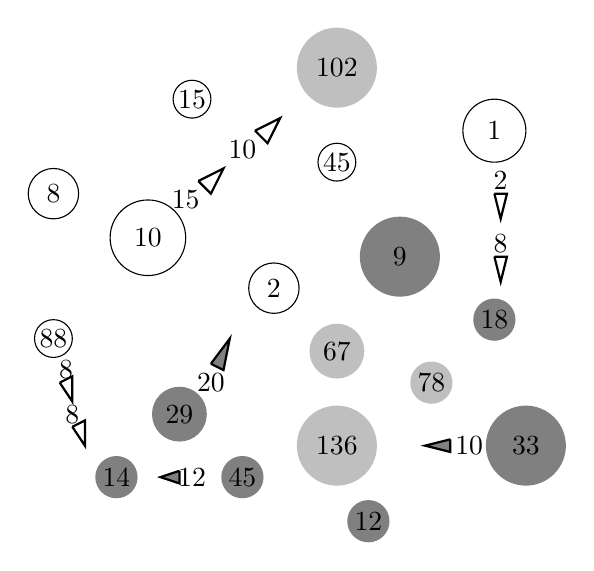
\begin{tikzpicture}[scale = 0.8]
\draw [fill =gray, ultra thick, gray] (2,1) circle [radius=0.3];
\node at (2,1) {14};
\draw [fill =gray, ultra thick, gray] (3,2) circle [radius=0.4];
\draw [fill = gray ,thick] (3.5,2.8) to (3.7,2.7) to (3.8,3.2) to (3.5,2.8);
\node at (3.5,2.5) {20};
\node at (3,2) {29};
\draw [fill =gray, ultra thick, gray] (4,1) circle [radius=0.3];
\node at (4,1) {45};
\draw [fill =gray ,thick] (3,1.1) to (3,0.9) to (2.7,1) to (3,1.1);
\node at (3.2,1) {12};
\draw [fill =gray, ultra thick, gray] (6,0.3) circle [radius=0.3];
\node at (6,0.3) {12};
\draw [fill =gray, ultra thick, gray] (8.5,1.5) circle [radius=0.6];
\node at (8.5,1.5) {33};
\draw [fill = gray ,thick] (7.3,1.6) to (6.9,1.5) to (7.3,1.4) to (7.3,1.6);
\node at (7.6,1.5) {10};
\draw [fill =gray, ultra thick, gray] (8,3.5) circle [radius=0.3];
\node at (8,3.5) {18};
\draw [fill =gray, ultra thick, gray] (6.5,4.5) circle [radius=0.6];
\node at (6.5,4.5) {9};
%\draw [fill =lightgray, ultra thick, lightgray] (3.5,3) circle [radius=0.3];
%\node at (3.5,3) {78};
\draw [fill =lightgray, ultra thick, lightgray] (5.5,1.5) circle [radius=0.6];
\node at (5.5,1.5) {136};
\draw [fill =lightgray, ultra thick, lightgray] (5.5,3) circle [radius=0.4];
\node at (5.5,3) {67};
\draw [fill =lightgray, ultra thick, lightgray] (7,2.5) circle [radius=0.3];
\node at (7,2.5) {78};
\draw [fill =lightgray, ultra thick, lightgray] (5.5,7.5) circle [radius=0.6];
\node at (5.5,7.5) {102};
\draw (1,3.2) circle [radius=0.3];
\node at (1,3.2) {88};
\draw [thick] (1.1,2.5) to (1.3,2.6) to (1.3,2.2) to (1.1,2.5);
\draw [thick] (1.3,1.8) to (1.5,1.9) to (1.5,1.5) to (1.3,1.8);
\node at (1.2,2.7) {8};
\node at (1.3,2) {8};
\draw  (1,5.5) circle [radius=0.4];
\node at (1,5.5) {8};
\draw  (2.5,4.8) circle [radius=0.6];
\node at (2.5,4.8) {10};
\draw  (3.2,7) circle [radius=0.3];
\draw [thick] (3.3,5.7) to (3.7,5.9) to (3.5,5.5) to (3.3,5.7);
\draw [thick] (4.2,6.5) to (4.6,6.7) to (4.4,6.3) to (4.2,6.5);
\node at (3.1,5.4) {15};
\node at (4,6.2) {10};
\node at (3.2,7) {15};
\draw  (4.5,4) circle [radius=0.4];
\node at (4.5,4) {2};
\draw  (5.5,6) circle [radius=0.3];
\node at (5.5,6) {45};
\draw  (8,6.5) circle [radius=0.5];
\draw [thick] (8,5.5) to (8.2,5.5) to (8.1,5.1) to (8,5.5);
\draw [thick] (8,4.5) to (8.2,4.5) to (8.1,4.1) to (8,4.5);
\node at (8,6.5) {1};
\node at (8.1,5.7) {2};
\node at (8.1,4.7) {8};
\end{tikzpicture}
\caption{an early stage of a planet wars game, as shown here there are planet categories, the darker grey (red in the game) ones related to the player, the white ones (green in the game) related to the opponent and the neutral planets are coloured by light grey. Fleets presented by triangles and the numbers are the starships included on them.}
\end{figure}

The environment of planet war forced to assign properties to every single object in the game.\cite{doc1} Such as, each planet in the map has two coordination points X and Y for its location, the ownerID, number of troops situated on it and the growth rate. To make an attack against enemies, the bot has to include starships and fleets under the attack. Each fleet has playerID, starships number included on it, source planetID, destination planetID and the number of turns need to achieve the goal, While the player is able to make one action per turn.\cite{doc1}

After each action, the planets will increase their ships number based on their growth rate.\cite{doc5} Moreover, if the source planet and the destination planet owner are the same ones, so we will consider that as a reinforcement by adding extra ships to the destination planet. Otherwise, if the target is a neutral planet, the bot has to calculate the exact starships need to win conquest the planet, whilst, if the target is an opponent, the two contenders will fight until one of them who has the highest number of starships will win the planet.\cite{doc1,doc5}

When the player makes an action and sends fleets, they can not change their direction until they will reach the destination they sent for it. As we mentioned previously, each match has a limited number of turns cannot go throw. So, by the end of the match, the player with the highest number of ships win the game. If one of them lose all their ships without finishing their total turns number, the game will complete faster, whilst, if the two players have the same number of troops, we have a draw.\cite{doc5}. 
\section{immune system overview}
The biology is one of the most inspirational domains that help the computational to solve many hard problems.\cite{doc7} Among the natural concepts, the immune system is one of the important aspects that provide several technics to design many optimization algorithms. An optimization problem\cite{doc6} is to search for the optimum solution from a set of potential solutions. The most algorithms used in this wide research are Heuristics.\cite{doc6} That include divers algorithms such as firefly swarm optimization, artificial bee colony, genetic algorithm, just to mention a few. While the Artificial Immune system (AIS)\cite{doc6} is a population-based algorithm. However, the application of the Artificial Immune System within technologies areas is a challenge is a self. Likewise, the researchers could exploit just a few immune's mechanisms because even in biology, this system still under a wide research area itself. 

\subsection{natural immune system}
The biological immune system including human system contains cells, molecules, and organs in the global structure to defend the body against diseases.\cite{doc6} The immune system has the ability to recognize the self-body cells and the nonself cells. In addition, this technic is very important to make an immune response by activating a suitable process to defeat the nonself cells.\cite{doc6} This response process will be activated according to antigens type, every antigene type activate a specific immune response process. whilst, memory cells are produced and activate when there is the same immune response type later.
\subsubsection*{Clonal selection}
To activate a response against the pathogens, the immune system uses multiple mechanisms. One of the interesting immune response is the clonal selection, this response type describes the process how the immune system can stimulus against a specific type of pathogens by proliferating a specific type of cells who can recognize the antigen.\cite{doc7} When a clonal selection response was stimulated, a specific type of cells (the B-cells) be proliferating according to affinity maturation, that's mean the high affinity will generate a hight clone number.
\begin{figure}
\centering
\begin{tabular}{c}
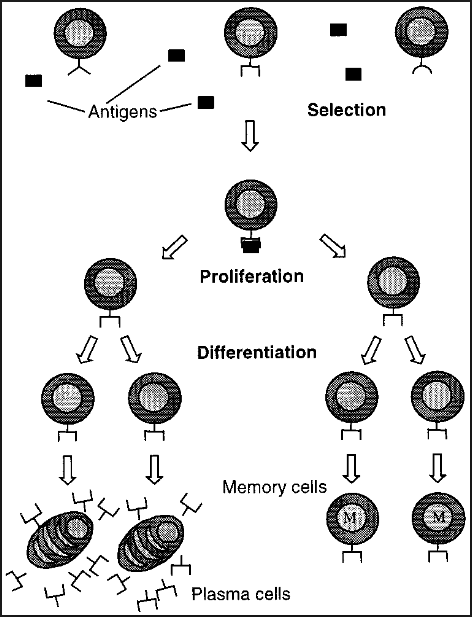
\includegraphics[scale = 0.8]{clonaS}
\end{tabular}
\caption{The biological clonal selection mechanism and its steps in order to defend the body, starting by detecting of the antigen until removing it.}
\end{figure}
The clonel selection process pass with multiple stps:
\paragraph{�}
The cloned cells undergo to a mutation process.
\paragraph{�}
the self-reactive receptor will be eliminated.
\paragraph{�}
proliferate the mature cells those can detect the antigen.

\subsection{Artificial Immune System}
In light of recent event in AIS, many algorithms have been developed trying to simulate ti clonal selection process. In 2002 Castro and Zuben proposed an optimization algorithm named CLONALG. The first step of this algorithm is to initialize an N random antibodies present the N potential solutions. in each iteration, the antibodies are cloned, mutated and selected the best of them preparing for the next generation. The proliferation of the antibodies is according to their affinities. While the maturation applied to equation (1): 
\begin{equation}
x_{id} = x_{id} + k(x_{d_{max}} - x_{d_{min}}) . N(0,1)
\end{equation}
where $x_{id}$ represent the dimension d of the antibody i, $x_{max}$ and $x_{min}$ represent the min and the max bounds of the variable i, N(0,1) is the standard distribution and k is the scale factor.

New random antibodies will be added to the original population by replacing a percentage of worsting antibodies and preparing to next generation.
\subsection{AIS pseudocode}
\begin{enumerate}
\item initialize N individual with random values between 0 and 1.
\item For iteration = 1 : maxIteration,
\begin{itemize}
\item Compute the affinities.
\item Clone the antibodies.
\item Mutate the antibodies cloned in the previous step.
\item Compute the affinities for the new antibodies mutated.
\item Applied the selection process to select the next generation
\end{itemize} 
End For \\
Display the optimal solutions. \\
End
\end{enumerate}
\begin{figure}
\centering
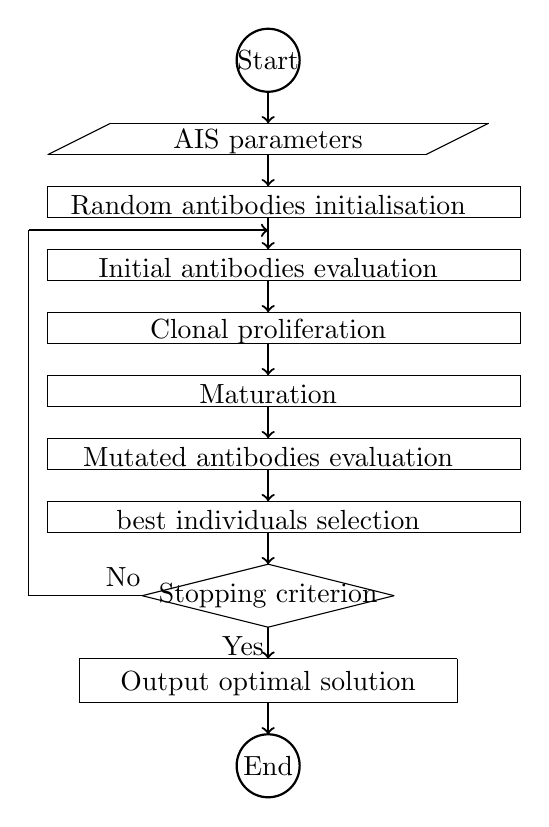
\begin{tikzpicture}[scale = 0.8]
\draw [thick] (4.5,20) circle [radius=0.5];
\node at (4.5,20) {Start};
\draw [->] [thick](4.5,19.5) -- (4.5,19);
\draw (2,19) --(8,19);
\draw (1,18.5) --(7,18.5);
\draw (2,19) --(1,18.5);
\draw (8,19) --(7,18.5);
\node at (4.5,18.7) {AIS parameters};
\draw [->] [thick](4.5,18.5) -- (4.5,18);
\draw (1,18) --(8.5,18);
\draw (1,17.5) --(8.5,17.5);
\draw (1,18) --(1,17.5);
\draw (8.5,18) --(8.5,17.5);
\node at (4.5,17.7) {Random antibodies initialisation};
\draw [->] [thick](4.5,17.5) -- (4.5,17);
\draw (1,17) --(8.5,17);
\draw (1,16.5) --(8.5,16.5);
\draw (1,17) --(1,16.5);
\draw (8.5,17) --(8.5,16.5);
\node at (4.5,16.7) {Initial antibodies evaluation};
\draw [->] [thick](4.5,16.5) -- (4.5,16);
\draw (1,16) --(8.5,16);
\draw (1,15.5) --(8.5,15.5);
\draw (1,15.5) --(1,16);
\draw (8.5,15.5) --(8.5,16);
\node at (4.5,15.7) {Clonal proliferation};
\draw [->][thick] (4.5,15.5) -- (4.5,15);
\draw (1,15) --(8.5,15);
\draw (1,14.5) --(8.5,14.5);
\draw (1,14.5) --(1,15);
\draw (8.5,14.5) --(8.5,15);
\node at (4.5,14.7) {Maturation};
\draw [->][thick] (4.5,14.5) -- (4.5,14);
\draw (1,14) --(8.5,14);
\draw (1,13.5) --(8.5,13.5);
\draw (1,13.5) --(1,14);
\draw (8.5,13.5) --(8.5,14);
\node at (4.5,13.7) {Mutated antibodies evaluation};
\draw [->][thick] (4.5,13.5) -- (4.5,13);
\draw (1,13) --(8.5,13);
\draw (1,12.5) --(8.5,12.5);
\draw (1,12.5) --(1,13);
\draw (8.5,12.5) --(8.5,13);
\node at (4.5,12.7) {best individuals selection};
\draw [->][thick] (4.5,12.5) -- (4.5,12);
\draw (4.5,12) --(2.5,11.5);
\draw (2.5,11.5) --(4.5,11);
\draw (4.5,11) --(6.5,11.5);
\draw (6.5,11.5) --(4.5,12);
\node at (4.5,11.5) {Stopping criterion};
\draw (2.5,11.5) --(0.7,11.5);
\draw (0.7,11.5) --(0.7,17.3);
\node at (4.1,10.7) {Yes};
\node at (2.2,11.8) {No};
\draw [->][thick] (0.7,17.3) -- (4.5,17.3);
\draw [->][thick] (4.5,11) -- (4.5,10.5);
\draw (1.5,10.5) --(7.5,10.5);
\draw (1.5,9.8) --(7.5,9.8);
\draw (1.5,10.5) --(1.5,9.8);
\draw (7.5,10.5) --(7.5,9.8);
\node at (4.5,10.1) {Output optimal solution};
\draw [->][thick](4.5,9.8) -- (4.5,9.3);
\draw [thick](4.5,8.8) circle [radius=0.5];
\node at (4.5,8.8) {End};
\end{tikzpicture}
\caption{The diagram showed the ordered steps for running an AIS algorithm based on clonal selection algorithm (CLONALG) }
\end{figure}

\subsection{Particle Swarm Optimization}
Recently, a considerable literature has grown up around the theme of swarm intelligence which plays an important role in addressing the issue of computational systems inspired its techniques from nature collective intelligence such us fish schooling, ants, flocks of birds to mention a few.
The algorithm run in a multi-dimensional space where all particles try to locate the optimum. By first, a set of a collection will be set to represent whole particles in the swarm randomly positioned in the working space, Each particle can move to find the potential optimum pathway according to the personal position of the particle (Pbest)  and the global position (Gbest) of all the swarm. In addition, another factor will influent this changing in the position, it's velocity. The change in velocity is measured with the equation (2):

\begin{equation}
v_{i}(t+1) = v_{i}(t) + c_{1}r_{1}(p_{i}^{Pbest}-p_{i}(t))  + c_{2}r_{2}(p_{Gbest}-p_{i}(t))
\end{equation}

Where $v_{i}(t+1)$ is the next velocity of the particle i, $c_{1}$ and $c_{2}$ represent the weight of Cognitive component and the Social component  for the personal best and global best successively. $p_{i}(t)$ is the position i of the particle p at time t. $p_{i}^{Pbest}$ is the best known position for the $i^{th}$ particle. $p_{Gbest}$ is the best known position for the whole swarm. $r_{1}$ and $r_{2}$ are random variables in the range [0, 1]. In the other side, the position for each particle  will be changed according to equation (3):

\begin{equation}
p_{i}(t+1) = p_{i}(t) + v_{i}(t)
\end{equation}

Where $p_{i}(t+1)$ represent the next position of the particle i.$p_{i}(t)$ is the current position of the particle i at time t and $v_{i}(t)$ is the velocity factor.

\section{AisBot: the Canquer Bot}

To design planet war conquest bot, you will face two major problems as we said in previous sections. The primary constraint is related to time, the bot has just 1 second to make an action. The second main problem is the memory restriction, the bot couldn't store any pieces of information from previous turns. This paper attempt to study these restrictions that limit the design performance of the bot's behaviour by using a set of rules in order to optimize the decision engine. \\

Anyway, the bot will perform one single action during the game is to make fleets move around the map from a planet to another. before the decision engine makes the bot move, it should distinguish between the self and the non-self planet. based on this simple action the greatest challenge is to determine which planet will generate fleets, how many starships will be included on it and which planet will be attacked. Next, we will describe the parameters used in the optimization following by the technics governing the bot.




\subsection{AisBot}
In order to improve our experimentations, we used the AisBot as a fighter bot during planet war game and it works as follow: The first step, the bot tries to determine the base planet using score function. Next, the bot tries to find a planet to send a fleet to it, if the target is an enemy, so the action made by the bot considered as a conquest. If the target planet is a colony, the action its a reinforcement; while, if the target owned by neutral, the action is taken as expansion. The fleets take more time to reach the target planet and cannot change their direction. Once the base planet will be reinforced by the colony, the action will be considered as a Tith. In addition, the colony can make an attack against the target planet if it is closer instead of sending starships to the base planet with the aim of attacking the target. Besides that, if a planet has been targeted, the bot can not decide an additional attack against the same planet till ending the first one.\\

When the attack mode is an expansion, the bot can know the exact number of starships need to win the planet, while, if the attack mode is a conquest, the bot should estimate the number of troops needs to defeat the enemy and quest the planet.

\begin{figure*}
\centering
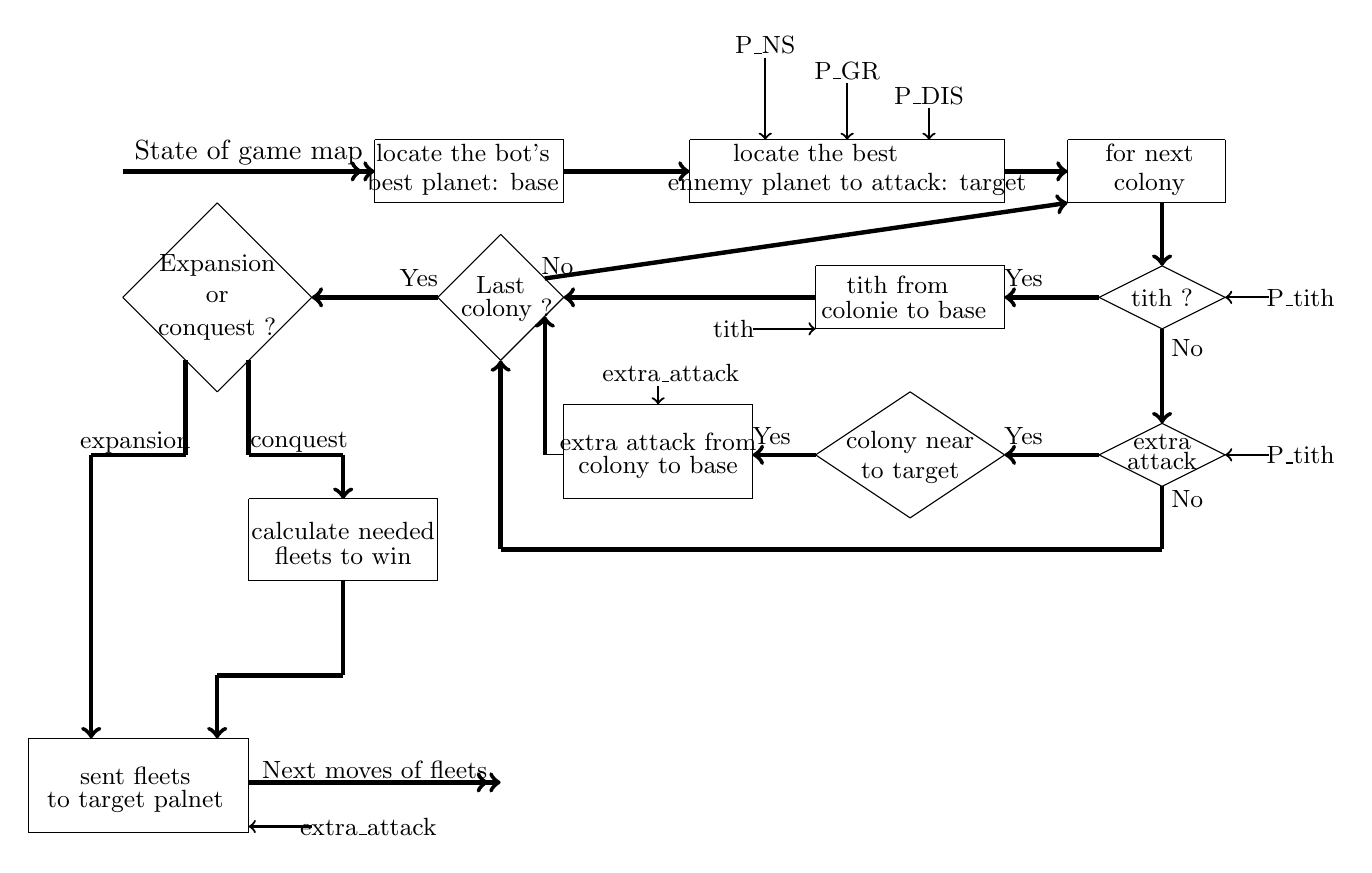
\begin{tikzpicture}[scale = 0.8]
\draw [->][ultra thick](-1,20) -- (3,20);
\draw [->][ultra thick](-1,20) -- (2.8,20);
\node at (1,20.3) {State of game map};
\draw (3,20.5) --(3,19.5);
\draw (3,20.5) --(6,20.5);
\draw (6,20.5) --(6,19.5);
\draw (6,19.5) --(3,19.5);
\draw [->][ultra thick](6,20) -- (8,20);
\node at (4.4,20.3) {\small locate the bot's};
\node at (4.4,19.8) {\small best planet: base};
\draw (8,20.5) --(8,19.5);
\draw (8,20.5) --(13,20.5);
\draw (13,20.5) --(13,19.5);
\draw (13,19.5) --(8,19.5);
\draw [->][thick](9.2,21.8) -- (9.2,20.5);
\draw [->][thick](10.5,21.4) -- (10.5,20.5);
\draw [->][thick](11.8,21) -- (11.8,20.5);
\node at (10,20.3) {\small locate the best};
\node at (9.2,22) {\small P\_NS};
\node at (10.5,21.6) {\small P\_GR};
\node at (11.8,21.2) {\small P\_DIS};
\node at (10.5,19.8) {\small ennemy planet to attack: target};
\draw [->][ultra thick](13,20) -- (14,20);
\draw (14,20.5) --(14,19.5);
\draw (14,20.5) --(16.5,20.5);
\draw (16.5,20.5) --(16.5,19.5);
\draw (16.5,19.5) --(14,19.5);
\node at (15.3,20.3) {\small for next};
\node at (15.3,19.8) {\small colony};
\draw [->][ultra thick](15.5,19.5) -- (15.5,18.5);
\draw (15.5,18.5) --(14.5,18);
\draw (14.5,18) --(15.5,17.5);
\draw (15.5,17.5) --(16.5,18);
\draw (16.5,18) --(15.5,18.5);
\draw [->][thick](17.2,18) -- (16.5,18);
\node at (17.7,18) {\small P\_tith};
\draw [->][thick](17.2,15.5) -- (16.5,15.5);
\node at (17.7,15.5) {\small P\_tith};
\node at (15.5,18) {\small tith ?};
\node at (15.5,15.7) {\small extra};
\node at (15.5,15.4) {\small attack};
\draw [->][ultra thick](15.5,17.5) -- (15.5,16);
\node at (15.9,17.2) {\small No};
\draw (15.5,16) --(14.5,15.5);
\draw (14.5,15.5) --(15.5,15);
\draw (15.5,15) --(16.5,15.5);
\draw (16.5,15.5) --(15.5,16);
\draw [->][ultra thick](14.5,18) -- (13,18);
\node at (13.3,18.3) {\small Yes};
\draw [ultra thick](15.5,15) -- (15.5,14);
\node at (15.9,14.8) {\small No};
\draw [ultra thick](15.5,14) -- (5,14);
\draw [->][ultra thick](5,14) -- (5,17);
\draw (13,18.5) --(13,17.5);
\draw (13,17.5) --(10,17.5);
\draw (10,17.5) --(10,18.5);
\draw (10,18.5) --(13,18.5);
\node at (13.3,15.8) {\small Yes};
\node at (11.3,18.2) {\small tith from};
\node at (11.4,17.8) {\small colonie to base};
\node at (8.7,17.5) {\small tith};
\draw [->][thick](9,17.5) -- (10,17.5);
\draw [->][ultra thick](14.5,15.5) -- (13,15.5);
\node at (9.3,15.8) {\small Yes};
\draw (13,15.5) --(11.5,16.5);
\draw (11.5,16.5) --(10,15.5);
\draw (10,15.5) --(11.5,14.5);
\draw (11.5,14.5) --(13,15.5);
\node at (11.5,15.7) {\small colony near};
\node at (11.5,15.2) {\small to target};
\draw [->][ultra thick](10,15.5) -- (9,15.5);
\draw (9,16.3) --(9,14.8);
\draw (9,14.8) --(6,14.8);
\draw (6,14.8) --(6,16.3);
\draw (6,16.3) --(9,16.3);
\node at (7.5,15.7) {\small extra attack from};
\node at (7.5,15.3) {\small colony to base};
\draw [->][thick](7.5,16.6) -- (7.5,16.3);
\node at (7.7,16.8) {\small extra\_attack};
\draw [->][ultra thick](10,18) -- (6,18);
\draw (6,18) --(5,19);
\draw (5,19) --(4,18);
\draw (4,18) --(5,17);
\draw (5,17) --(6,18);
\node at (5,18.2) {\small Last};
\node at (5.1,17.8) {\small colony ?};
\draw [->][ultra thick](5.7,18.3) -- (14,19.5);
\node at (5.9,18.5) {\small No};
\node at (3.7,18.3) {\small Yes};
\draw (6,15.5) -- (5.7,15.5);
\draw [->][ultra thick](5.7,15.5) -- (5.7,17.7);
\draw [->][ultra thick](4,18) -- (2,18);
\draw (2,18) -- (0.5,19.5);
\draw (0.5,19.5) -- (-1,18);
\draw (-1,18) -- (0.5,16.5);
\draw (0.5,16.5) -- (2,18);
\node at (0.5,18.5) {\small Expansion };
\node at (0.5,18) {\small or };
\node at (0.5,17.5) {\small conquest ?};
\draw [ultra thick](1,17) -- (1,15.5);
\draw [ultra thick](1,15.5) -- (2.5,15.5);
\node at (1.8,15.7) {\small conquest};
\draw [->][ultra thick](2.5,15.5) -- (2.5,14.8);
\draw (1,14.8) -- (4,14.8);
\draw (4,14.8) -- (4,13.5);
\draw (4,13.5) -- (1,13.5);
\draw (1,13.5) -- (1,14.8);
\node at (2.5,14.3) {\small calculate needed};
\node at (2.5,13.9) {\small fleets to win};
\draw [ultra thick](0,17) -- (0,15.5);
\draw [ultra thick](0,15.5) -- (-1.5,15.5);
\draw [->][ultra thick](-1.5,15.5) -- (-1.5,11);
\draw (-2.5,11) -- (1,11);
\draw (-2.5,9.5) -- (1,9.5);
\draw (-2.5,11) -- (-2.5,9.5);
\draw (1,11) -- (1,9.5);
\draw [ultra thick](2.5,13.5) -- (2.5,12);
\draw [ultra thick](2.5,12) -- (0.5,12);
\node at (-0.8,15.7) {\small expansion};
\draw [->][ultra thick](0.5,12) -- (0.5,11);
\node at (-0.8,10.4) {\small sent fleets};
\node at (-0.8,10) {\small to target palnet};
\draw [->][ultra thick](1,10.3) -- (4.8,10.3);
\draw [->][ultra thick](1,10.3) -- (5,10.3);
\node at (3,10.5) {\small Next moves of fleets};
\draw [->][thick](2,9.6) -- (1,9.6);
\node at (2.9,9.6) {\small extra\_attack};
\end{tikzpicture}
\caption{The states that are governing the behaviour of the AisBot including the parameters used on the evaluation of the bot's behaviour. these parameters will improve by the clonal selection algorithm (CLONALG).}
\end{figure*}

%If your manuscript has supplementary content you can also use the \verb"interact" class file to prepare all or part of it using the \verb"suppldata" document-class option, which will suppress the `article history' date. This option \emph{must not} be used on any primary content. Note that authors are solely responsible for the preparation of all supplemental material.


\begin{figure*}
\centering
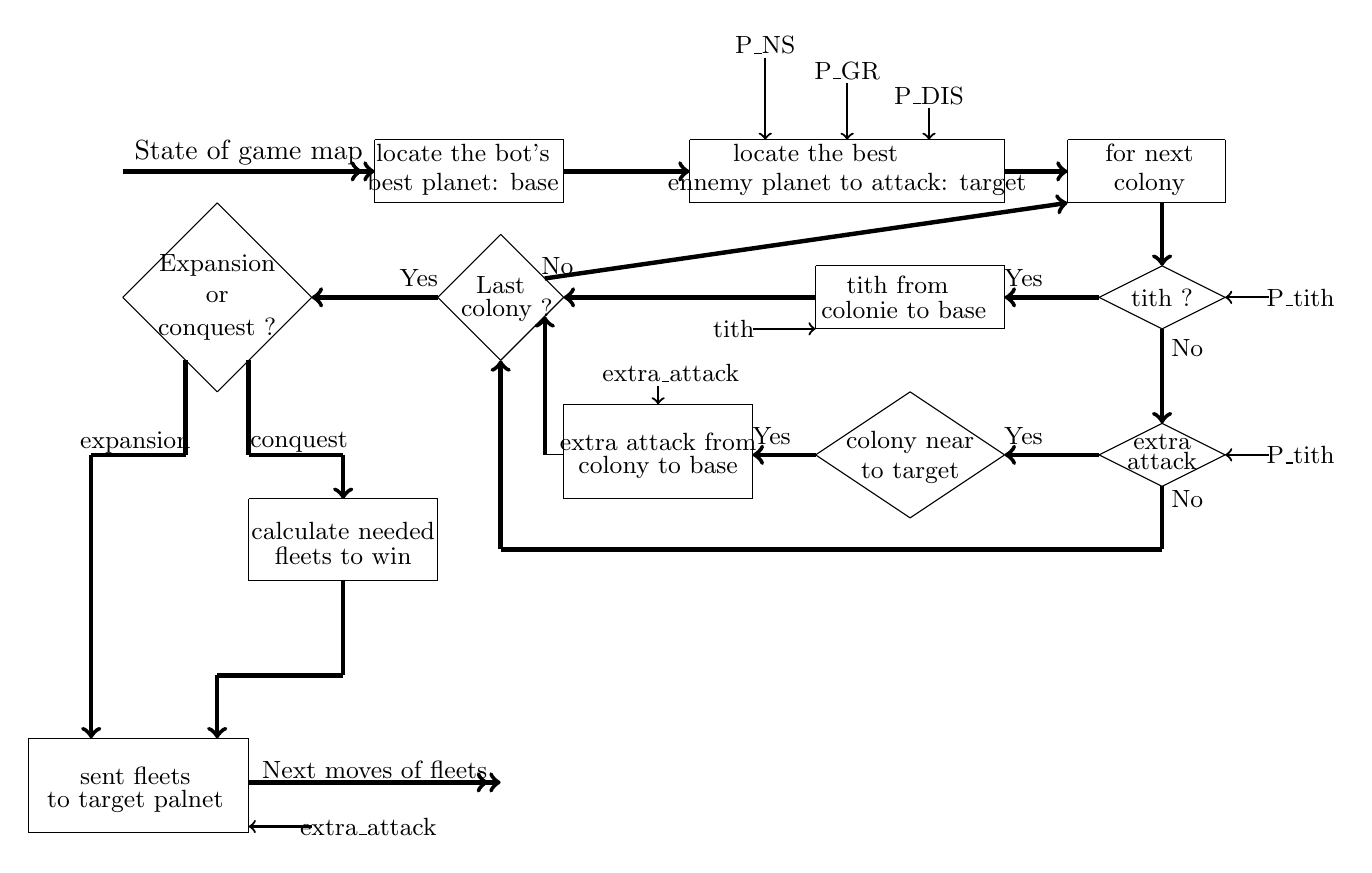
\begin{tikzpicture}[scale = 0.8]
\draw [->][ultra thick](-1,20) -- (3,20);
\draw [->][ultra thick](-1,20) -- (2.8,20);
\node at (1,20.3) {State of game map};
\draw (3,20.5) --(3,19.5);
\draw (3,20.5) --(6,20.5);
\draw (6,20.5) --(6,19.5);
\draw (6,19.5) --(3,19.5);
\draw [->][ultra thick](6,20) -- (8,20);
\node at (4.4,20.3) {\small locate the bot's};
\node at (4.4,19.8) {\small best planet: base};
\draw (8,20.5) --(8,19.5);
\draw (8,20.5) --(13,20.5);
\draw (13,20.5) --(13,19.5);
\draw (13,19.5) --(8,19.5);
\draw [->][thick](9.2,21.8) -- (9.2,20.5);
\draw [->][thick](10.5,21.4) -- (10.5,20.5);
\draw [->][thick](11.8,21) -- (11.8,20.5);
\node at (10,20.3) {\small locate the best};
\node at (9.2,22) {\small P\_NS};
\node at (10.5,21.6) {\small P\_GR};
\node at (11.8,21.2) {\small P\_DIS};
\node at (10.5,19.8) {\small ennemy planet to attack: target};
\draw [->][ultra thick](13,20) -- (14,20);
\draw (14,20.5) --(14,19.5);
\draw (14,20.5) --(16.5,20.5);
\draw (16.5,20.5) --(16.5,19.5);
\draw (16.5,19.5) --(14,19.5);
\node at (15.3,20.3) {\small for next};
\node at (15.3,19.8) {\small colony};
\draw [->][ultra thick](15.5,19.5) -- (15.5,18.5);
\draw (15.5,18.5) --(14.5,18);
\draw (14.5,18) --(15.5,17.5);
\draw (15.5,17.5) --(16.5,18);
\draw (16.5,18) --(15.5,18.5);
\draw [->][thick](17.2,18) -- (16.5,18);
\node at (17.7,18) {\small P\_tith};
\draw [->][thick](17.2,15.5) -- (16.5,15.5);
\node at (17.7,15.5) {\small P\_tith};
\node at (15.5,18) {\small tith ?};
\node at (15.5,15.7) {\small extra};
\node at (15.5,15.4) {\small attack};
\draw [->][ultra thick](15.5,17.5) -- (15.5,16);
\node at (15.9,17.2) {\small No};
\draw (15.5,16) --(14.5,15.5);
\draw (14.5,15.5) --(15.5,15);
\draw (15.5,15) --(16.5,15.5);
\draw (16.5,15.5) --(15.5,16);
\draw [->][ultra thick](14.5,18) -- (13,18);
\node at (13.3,18.3) {\small Yes};
\draw [ultra thick](15.5,15) -- (15.5,14);
\node at (15.9,14.8) {\small No};
\draw [ultra thick](15.5,14) -- (5,14);
\draw [->][ultra thick](5,14) -- (5,17);
\draw (13,18.5) --(13,17.5);
\draw (13,17.5) --(10,17.5);
\draw (10,17.5) --(10,18.5);
\draw (10,18.5) --(13,18.5);
\node at (13.3,15.8) {\small Yes};
\node at (11.3,18.2) {\small tith from};
\node at (11.4,17.8) {\small colonie to base};
\node at (8.7,17.5) {\small tith};
\draw [->][thick](9,17.5) -- (10,17.5);
\draw [->][ultra thick](14.5,15.5) -- (13,15.5);
\node at (9.3,15.8) {\small Yes};
\draw (13,15.5) --(11.5,16.5);
\draw (11.5,16.5) --(10,15.5);
\draw (10,15.5) --(11.5,14.5);
\draw (11.5,14.5) --(13,15.5);
\node at (11.5,15.7) {\small colony near};
\node at (11.5,15.2) {\small to target};
\draw [->][ultra thick](10,15.5) -- (9,15.5);
\draw (9,16.3) --(9,14.8);
\draw (9,14.8) --(6,14.8);
\draw (6,14.8) --(6,16.3);
\draw (6,16.3) --(9,16.3);
\node at (7.5,15.7) {\small extra attack from};
\node at (7.5,15.3) {\small colony to base};
\draw [->][thick](7.5,16.6) -- (7.5,16.3);
\node at (7.7,16.8) {\small extra\_attack};
\draw [->][ultra thick](10,18) -- (6,18);
\draw (6,18) --(5,19);
\draw (5,19) --(4,18);
\draw (4,18) --(5,17);
\draw (5,17) --(6,18);
\node at (5,18.2) {\small Last};
\node at (5.1,17.8) {\small colony ?};
\draw [->][ultra thick](5.7,18.3) -- (14,19.5);
\node at (5.9,18.5) {\small No};
\node at (3.7,18.3) {\small Yes};
\draw (6,15.5) -- (5.7,15.5);
\draw [->][ultra thick](5.7,15.5) -- (5.7,17.7);
\draw [->][ultra thick](4,18) -- (2,18);
\draw (2,18) -- (0.5,19.5);
\draw (0.5,19.5) -- (-1,18);
\draw (-1,18) -- (0.5,16.5);
\draw (0.5,16.5) -- (2,18);
\node at (0.5,18.5) {\small Expansion };
\node at (0.5,18) {\small or };
\node at (0.5,17.5) {\small conquest ?};
\draw [ultra thick](1,17) -- (1,15.5);
\draw [ultra thick](1,15.5) -- (2.5,15.5);
\node at (1.8,15.7) {\small conquest};
\draw [->][ultra thick](2.5,15.5) -- (2.5,14.8);
\draw (1,14.8) -- (4,14.8);
\draw (4,14.8) -- (4,13.5);
\draw (4,13.5) -- (1,13.5);
\draw (1,13.5) -- (1,14.8);
\node at (2.5,14.3) {\small calculate needed};
\node at (2.5,13.9) {\small fleets to win};
\draw [ultra thick](0,17) -- (0,15.5);
\draw [ultra thick](0,15.5) -- (-1.5,15.5);
\draw [->][ultra thick](-1.5,15.5) -- (-1.5,11);
\draw (-2.5,11) -- (1,11);
\draw (-2.5,9.5) -- (1,9.5);
\draw (-2.5,11) -- (-2.5,9.5);
\draw (1,11) -- (1,9.5);
\draw [ultra thick](2.5,13.5) -- (2.5,12);
\draw [ultra thick](2.5,12) -- (0.5,12);
\node at (-0.8,15.7) {\small expansion};
\draw [->][ultra thick](0.5,12) -- (0.5,11);
\node at (-0.8,10.4) {\small sent fleets};
\node at (-0.8,10) {\small to target palnet};
\draw [->][ultra thick](1,10.3) -- (4.8,10.3);
\draw [->][ultra thick](1,10.3) -- (5,10.3);
\node at (3,10.5) {\small Next moves of fleets};
\draw [->][thick](2,9.6) -- (1,9.6);
\node at (2.9,9.6) {\small extra\_attack};
\end{tikzpicture}
\caption{The states that are governing the behaviour of the AisBot including the parameters used on the evaluation of the bot's behaviour. these parameters will improve by the clonal selection algorithm (CLONALG).}
\end{figure*}

%%\includepdf[scale=0.7,pages=1]{botDiagram}


As we mentioned previously, the purpose of this study is to try to optimize the behaviour of a bot during the planet war RTS game. In order to improve our experimentation, we use the AisBot as a conquer bot in this game, and it works as follows: first of all, when a turn is started, the bot tries to determine the base planet based on a score function and the rest of planets are used as colonies.Secondly, the bot decides which planet to attack for the next turn or if it owns additional planet the action will be considered as a reinforcement, in order to reach the target planet, it can take some number of turns. If the bot trying to attack a target is owned by a neutral, the action will be considered as an expansion; however, if it's owned by the enemy, the action will be considered as a conquest. Once the base planet is reinforced by starships coming from colonies, the action will be considered as a Tith. In addition, when colonies that are closed to the target planet than the base is allowed to attack the target by sending fleets, instead of reinforcing the base and this one sends those fleets to the target planet, but move directly to the target. Besides, when a planet was targeted by the bot, it is no possible to decide another attack against the same planet until the first one finished, that is mean, for each fleet sent to perform an attack, it knows the target planet in its data structure. \\

In order to improve the behaviour of the bot,  a set of rules is defined included some parameters classified by weights, probabilities and amounts. the parameters signification is : 
\begin{itemize}
\item \textit{$Tith_{perc}$}: starships proportions that the bot can sends.
\item \textit{$Tith_{prob}$}: Tith probability that a colony sends to the base planet.
\item \textit{$w_{NS}$}: weight of starships number hosted on the planet.
\item \textit{$w_{DIS}$}: weight of distance between the base and the target planet.
\item \textit{$w_{GR}$}: weight of growth rate according to the target planet.
\item \textit{$Pool_{perc}$}: percentage of extra starships can send from the base to the target planet.
\item \textit{$Support_{perc}$}: Percentage of extra starships from the colony to the target.
\item \textit{$Support_{prob}$}: Probability of sending extra starships from the colony to the target.
\end{itemize}
Furthermore, each parameter takes some values during the optimization process depends on it meaning in the game, our conquer bot will be based on these values to make decisions during the game. To determine the target planet the bot will use a score function define as follow:

\begin{equation}
Score(p) = \frac{p.NumStarships.w_{NS-DIS}.Dist(base,p)}{1+p.GrowthRate.w_{GR}}
\end{equation}

Where the $w_{NS-dis}$ and the $w_{GR}$ are weights related successively to starships number, the growth rate for the planet and the distance to reach the target. As we mentioned above the $base$ is the planet which has the highest number of starships and $p$ refer to planet want to evaluate. \\ 

When the Tith and the attack process are performed by the colonies, the base planet also sends starships to attack the target. The number of starships sends to attack is estimated according to the attack mode, if the bot attack mode is expansion where the target does not generate starships during the game that implies the bot will integrate a very specific starships number to be able to defeat the planet target, in the other hand, if the bot attack mode is a conquest, the engine will estimate the number of troops needs to beat the enemy.
\section{AisBot: an AIS optimization}
The purpose of our optimization is to make the bot move faster and try to minimize the number of turns before destroying the enemy. In the other hand, a CLONALG algorithm will be applied in the set of parameters that will determine the behaviour of the bot, once the parameters are improved, the bot will upload them in order to go under real game scenarios. \\

Therefore, the purpose is to determine the parameters values in order to evaluate the bot's behaviour.The AIS proposed in this study use a floating array to represent all parameters defined previously, while, the clonal proliferation process works on a totally new array with a specific proliferation factor for each parameter according to its fitness. The maturation mechanism is applied to the cloned antibodies by mutating the parameters values using the equation (1) with a probability amount to minimize the bad antibodies. \\

The selection process based on an evaluation technic by implementing tournaments where each cloned individual used to compete with the aim of being selected for the next generation from the best results were chosen. The evaluation of an individual is staged by including their parameters for the AisBot behaviour and placing the bot on a real planet war game against the RandomBot on five maps. \\

The aim of this optimization is to minimize the number of turns needs to win, the best bot is the one that plays fewer turns until win; this kind of ranking bots strongly shown a constraint problem is that each individual was able to win every single game.

\section{Exprementation and results}
With the aim of testing the CLONALG algorithm, the bot placed under several situations and play several games against the RandomBot. The algorithm parameters can be found on the Table 1:
\begin{table}[h!]
\centering
\begin{tabular}{ |c|c| }
\hline
 Number of antibodies & 20 \\ 
 Number of generations & 15 \\  
 maximun antbodies Cloned & 72 \\ 
 \hline   
\end{tabular}
\caption{Parameters used in the CLONALG algorithm}
\label{TABLE 1}
\end{table}


To make a bot under a real game scenario with optimized parameters will take hours, since, to evaluate each individual it took more seconds. The figure (5) showed the evaluation of the number of turns plays by the bot until win, and it appears that the number of turns needs to win in five maps decrease. \\

\begin{comment}
\begin{figure}
\begin{center}
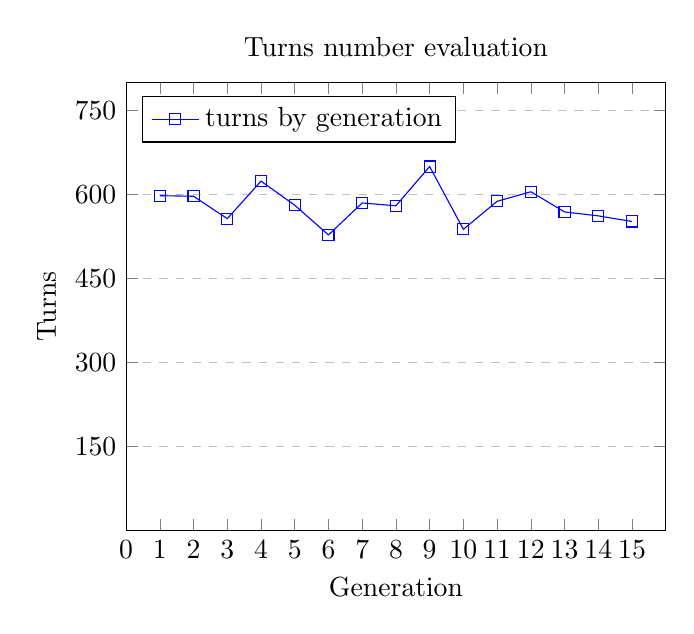
\begin{tikzpicture}
\begin{axis}[
    title={Turns number evaluation},
    xlabel={Generation},
    ylabel={Turns},
    xmin=0, xmax=16,
    ymin=0, ymax=800,
    xtick={0,1,2,3,4,5,6,7,8,9,10,11,12,13,14,15},
    ytick={150,300,450,600,750},
    legend pos=north west,
    ymajorgrids=true,
    grid style=dashed,
]
 
\addplot[
    color=blue,
    mark=square,
    ]
    coordinates {
    (1,598)(2,597)(3,557)(4,624)(5,581)(6,528)(7,585)(8,580)(9,650)(10,538)(11,588)(12,605)(13,569)(14,562)(15,552)
    };
    \legend{turns by generation}
 
\end{axis}
\end{tikzpicture}
\end{center}
\caption{the evaluation of the number of turns plays by the bot until win in 5 maps, and it appears that the number of turns needs to win in five maps decrease after the evaluation process}
\end{figure}
\end{comment}

\begin{figure}
\begin{center}
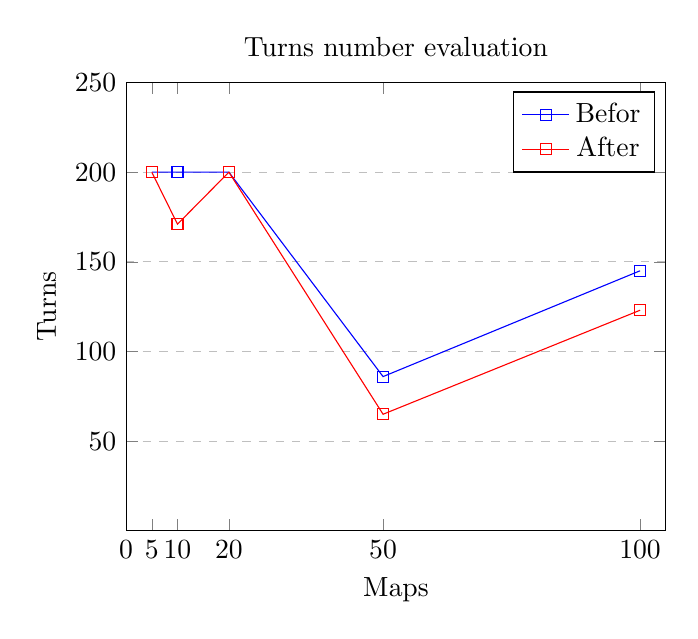
\begin{tikzpicture}
\begin{axis}[
    title={Turns number evaluation},
    xlabel={Maps},
    ylabel={Turns},
    xmin=0, xmax=105,
    ymin=0, ymax=250,
    xtick={0,5,10,20,50,100},
    ytick={50,100,150,200,250},
   % legend pos=outer north east,
    ymajorgrids=true,
    grid style=dashed,
]
 
\addplot[
    color=blue,
    mark=square,
    ]
    coordinates{(5,200)(10,200)(20,200)(50,86)(100,145)};
    
    \addplot[
    color=red,
    mark=square,
    ]
    coordinates{(5,200)(10,171)(20,200)(50,65)(100,123)};
    
    
    \legend{Befor, After}
 
\end{axis}
\end{tikzpicture}
\end{center}
\caption{The evaluation of the turns number needed to win around multiple maps between initial bot and optimized bot}
\end{figure}



Figure (6) and figure (7) describes the evaluated results improved by the optimization process where the colonies have a high probability to send Tith to the base (0.61) by sending a fewer hosted starships which can be explained that the colonies have to deserve there starships to defend it-selves in an emergency. On the other hand, the probability for a planet to perform an attack against other ones is around (0.42) and the proportion of sending troops is elevated (50\%) when there is an attack action. Based on this, when a planet performs an attack, the base also can send a high extra starships number for the attack around 43\%. Finally, when the bot trying to determine the target planet to perform the attack, the most important weights based on is the number of starships hosted on the target and the growth rate related to it, the distance has a less priority in this process. \\

\begin{comment}
\begin{table*}
\centering
\begin{tabular}{|c|c|c|c|c|c|c|c|c|}
\hline
 & $Tith_perc$ & $Tith_prob$ & $W_NS$ & $W_GR$ & $W_DIS$ & $Pool_perc$ & $Support_perc$ & $Support_prob$ \\ 
 \hline
 Before & 0.959 & 0.651 & 0.665 & 0.122 & 0.785 & 0.113 & 0.64 & 0.366 \\  
 \hline
 After & 0.057 & 0.845 & 0.447 & 0.323 & 0.124 & 0.814 & 0.636 & 0.32 \\
 \hline  
\end{tabular}
\caption{Parameters used in the CLONALG algorithm}
\label{TABLE 2}
\end{table*}
\end{comment}

%0.505,0.778,0.1,0.933,0.562,0.12,0.075,0.829

\begin{figure}
\begin{center}
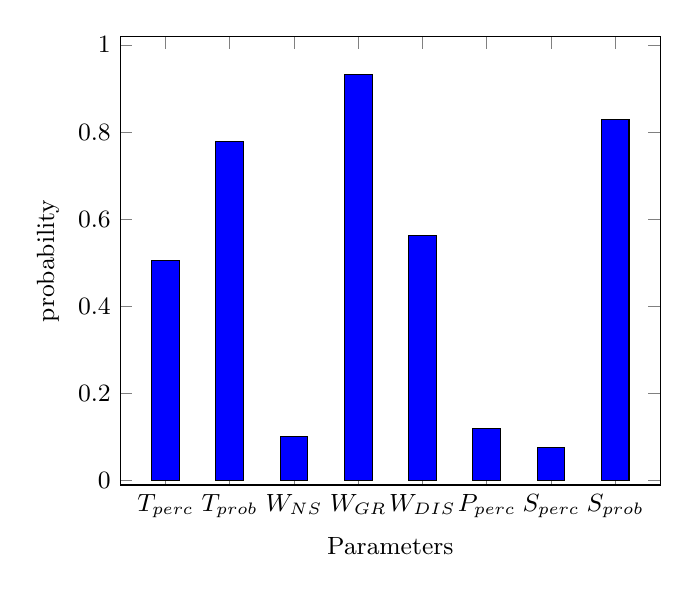
\begin{tikzpicture}[font=\small]
\begin{axis}[
    symbolic x coords={$T_{perc}$, $T_{prob}$, $W_{NS}$, $W_{GR}$, $W_{DIS}$, $P_{perc}$, $S_{perc}$, $S_{prob}$},
        ylabel = {probability},
        xlabel = {Parameters},
    xtick=data]
    \addplot[ybar,fill=blue] coordinates {
        ($T_{perc}$,0.505)
        ($T_{prob}$,0.778)
        ($W_{NS}$,0.1)
    ($W_{GR}$, 0.933)
    ($W_{DIS}$,0.562)
    ($P_{perc}$,0.12)
    ($S_{perc}$,0.075)
    ($S_{prob}$,0.829)
    };
\end{axis}
\end{tikzpicture}
\end{center}
\caption{The parameters values setting for the inital bot}
\end{figure}

%0.24,0.611,0.819,0.6,0.262,0.436,0.504,0.424

\begin{figure}
\begin{center}
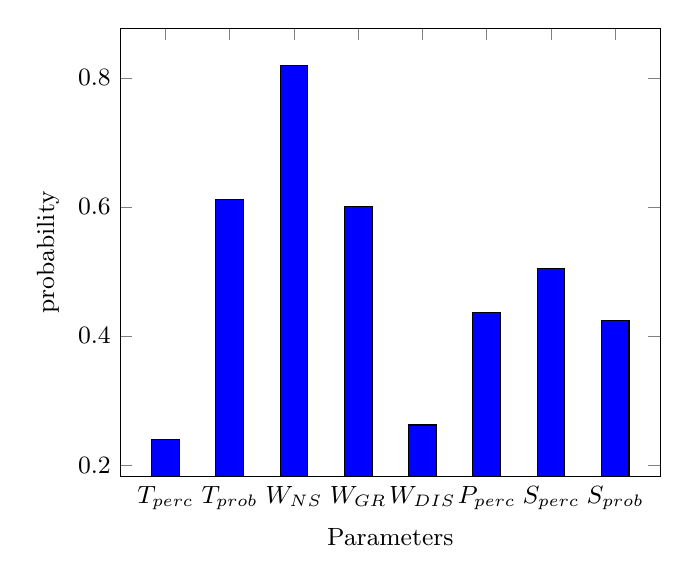
\begin{tikzpicture}[font=\small]
\begin{axis}[
    symbolic x coords={$T_{perc}$, $T_{prob}$, $W_{NS}$, $W_{GR}$, $W_{DIS}$, $P_{perc}$, $S_{perc}$, $S_{prob}$},
        ylabel = {probability},
        xlabel = {Parameters},
    xtick=data]
    \addplot[ybar,fill=blue] coordinates {
        ($T_{perc}$,0.24)
        ($T_{prob}$,0.611)
        ($W_{NS}$,0.819)
    ($W_{GR}$, 0.6)
    ($W_{DIS}$,0.262)
    ($P_{perc}$,0.436)
    ($S_{perc}$,0.504)
    ($S_{prob}$,0.424)
    };
\end{axis}
\end{tikzpicture}
\end{center}
\caption{The parameters values setting for the optimized bot}
\end{figure}

\begin{comment}
\begin{table*}
\centering
\begin{tabular}{|c|c|c|c|c|c|}
\hline
 Maps & 5 & 10 & 20 & 50 & 100 \\ 
 \hline
 Before & 135 & 128 & 161 & 102 & 144 \\  
 \hline
 After & 98 & 80 & 70 & 72 & 87 \\
 \hline  
\end{tabular}
\caption{results after 5 games of our AisBot with random parameters and after the optimization against the RandomBot}
\label{TABLE 3}
\end{table*}
\end{comment}

In general, the optimised AisBot is able to defeat the DualBot in all situations with a minimum number of turns, this can demonstrate that the application of an Evolutionary Algorithm reach some hight capabilities in optimization behaviour even a parametrize behaviour as the one used on the AisBot. There are a lot of challenges can explore all the capabilities of AIS algorithms in the design of the bot's behaviour can offer.


\section{conclusions}
The planet wars game it was classified as an RTS game, where the player (bots) fight against others in real-time. The main aim of this study is to investigate the application of the Evolutionary Algorithms (EAs) and the better results can be obtained in real-world problems, by tunning real game scenarios that used a parametrise behaviour of a bot tuning by an AIS Algorithm. This problem showed that the EAs can improve the evaluation of a hand-coded bot by defeating multiple opponents in different situations in fewer turns. In the other hand, the high capabilities of an evolutionary approach can be improved at least in this type of problems.

\bibliography{references}

\addcontentsline{toc}{section}{Bibliography}

\bibliographystyle{abbrv}

\end{document}
